\lecture{19}{Dilute Solutions}{Qiang Zhu}{scribe-name1,2,3}

The solution is similar to the case of a mixture. A solution is called \textit{dilute} if the concentration of solute is much less than the number of solvents. In many ways the solute in a dilute solution behaves like an ideal gas. We can therefore predict many of the properties quantitatively.

\section{Solvent and Solute}
To make a prediction, we first need to know something about its chemical potentials. The chemical potential $\mu_A$ is related to the Gibbs free energy by $\mu_A = \partial G/\partial N_A$. Suppose we start with a pure solvent of $A$ molecules, then the Gibbs free energy is just $N_A$ times the chemical potential.

\begin{equation}
G = N_A\mu_0(T, P)  ~~~~~~~~ \textrm{(in pure solvent)}    
\end{equation}

where, $\mu_0$ is the chemical potential of the pure solvent, a function of temperature and pressure.

Now imagine that we add a single B molecule to the system by holding T and P fixed, the change in G can be expressed as follows,
\begin{equation}
dG = dU + PdV - TdS    
\end{equation}

While $dU$ and $PdV$ won't depend on $N_A$, $TdS$ term is sensitive to such change. The increase in S can be considered as proportional to $N_A$ 
\begin{equation}
dS = k\ln N_A     
\end{equation}

\begin{equation}
dG = f(T, P) - kT\ln N_A   ~~~~~(\textrm{adding one molecule B})  
\end{equation}

If we add two B molecules, 

\begin{equation}
dG = 2f(T, P) - 2kT\ln N_A + kT\ln2  ~~~~~(\textrm{adding one molecule B})  
\end{equation}
Note that we add the term of $\ln2$ due to the double counting of two B states.

\begin{equation}
G = N_A\mu_0(T, P) + N_Bf(T, P) - N_BkT\ln N_A  + N_BkT\ln N_B - N_BkT  
\end{equation}
This expression is valid when $N_B \ll N_A$. The solvent and solution chemical potential can be derived as follows

\begin{equation}
\mu_A = \frac{\partial G}{\partial N_A}_{T, P, N_B} = \mu_0(T, P) - \frac{N_BkT}{N_A}  
\end{equation}
\begin{equation}
\mu_B = \frac{\partial G}{\partial N_B}_{T, P, N_A} = \mu_0(T, P) - kT\ln(N_B/N_A)  
\end{equation}

As we would expect, adding more solute reduces the chemical potential of A and increase the chemical potential of B. Moreover, the results depend only on the ration of $N_B/N_A$. We can therefore define a quantity as molality ($m_B$). 
\begin{equation}\label{mub}
\mu_B = \mu^0(T, P) - kT\ln m_B  
\end{equation}

\section{Osmotic Pressure}
Consider a solution that is separated from some pure solvent by a membrane that allows only solvent molecules to pass through. According to eq(\ref{mub}), the chemical potential of the solvent in the solution is less than that of the pure solvent. Paticles tend to flow toward lower chemical potential, so the solvent molecules will spontaneously flow from the pure solvent into the solution. This flow of molecules is called \textbf{osmosis}. That osmosis should happen is counter-intuitive. 

If you want to 
\begin{equation}\label{mub}
\mu_0(T, P_1) = \mu_0(T, P_2) - \frac{N_BkT}{N_A}  
\end{equation}

where $P_1$ is the pressure on the side with pure solvent and $P_2$ is the pressure on the side of solution. Assuming that these two pressures are not too different, we can approximate
\begin{equation}\label{mub}
\mu_0(T, P_2) \approx \mu_0(T, P_1) - (P_2 - P_1) \frac{\partial \mu_0}{\partial P}  
\end{equation}

\begin{equation}
    (P_2 - P_1)\frac{\partial \mu_0}{\partial P} = \frac{N_BkT}{N_A}
\end{equation}

To evaluate the derivative $\frac{\partial \mu_0}{\partial P}$, we use $\mu = G/N$, so it is $V/N$. 
Therefore, the previous equation becomes,
\begin{equation}
    P_2 - P_1 = \frac{N_BkT}{V} = \frac{n_BRT}{V}
\end{equation}

This pressure different is called the osmotic pressure, and the formula is called \textbf{van't Hoff's formula}. It says that the osmotic pressure is exactly the same as the pressure of an ideal gas of the same concentration as the solute. This is useful for biophysics studies. 

\section{Boiling and Freezing Points}
Similar to the mixture of two phases, the concentration of solutes can shift the boiling and freezing points as well. Consider the case of a dilute solution at its boiling point, when it is in equilibrium with its gas phase (Fig. \ref{boil}). Assuming

\begin{equation}
    \mu_{\textrm{A, liq}}(T, P) = \mu_{\textrm{A, gas}}(T, P)
\end{equation}

Using the previous learned relation,
\begin{equation}
    \mu_0(T, P) - \frac{N_BkT}{N_A} = \mu_{\textrm{gas}}(T, P)
\end{equation}
where $\mu_0$ is the chemical potential of the pure solvent.
Now, as in the osmitic ***
\begin{equation}
    \mu_0(T, P_0) = \mu_{\textrm{gas}}(T, P_0)
\end{equation}

\begin{equation}
    \mu_0(T, P_0) + (P-P_0) \frac{\partial \mu_0}{\partial P} - \frac{N_BkT}{N_A} = \mu_{\textrm{gas}} (T, P_0) + (P-P_0) \frac{\mu_{\textrm{gas}}}{\partial P}
\end{equation}

\begin{equation}
    (P-P_0) \frac{V}{N} - \frac{N_BkT}{N_A} = (P-P_0) \bigg(\frac{V}{N}_{\textrm{gas}}\bigg)
\end{equation}

This can be reduced to

\begin{equation}
    P - P_0 = \frac{-N_B}{N_A} P_0, ~~~~~~~~~~~~~~~~~~ \frac{P}{P_0} = 1-\frac{N_B}{N_A}
\end{equation}

Alternatively, we could hold the pressure fixed and solve for the shift in temperature needed to maintian equilibrium in the presence of the solute. Let $T_0$ be the boiling point of the pure solvent at $P$, so that
\begin{equation}
    \mu_0(T_0, P) = \mu_{\textrm{gas}}(T_0, P)
\end{equation}

In terms of the chemical potentials at $T_0$. it becomes,
\begin{equation}
    \mu_0(T_0, P) + (T-T_0)\frac{\partial mu_0}{\partial T} - \frac{N_B kT}{N_A} = \mu_\textrm{gas}(T_0, P) + (T-T_0)\frac{\partial \mu_{\textrm{gas}}}{\partial T}
\end{equation}

Again the first term on each side cancels. Each $\partial mu/ \partial T$ is just minus $-S$, so
\begin{equation}
    -(T - T_0)\bigg(\frac{S}{N}\bigg)_\textrm{liq} - \frac{N_BkT}{N_A} = -(T-T_0)\bigg(\frac{S}{N}\bigg)_\textrm{gas}
\end{equation}
\begin{equation}
    T - T_0 = \frac{N_BkT_0^2}{L} = \frac{n_BRT_9^2}{L}
\end{equation}

With the results, let's compute the boiling temperature of seawater. A convenient quantity to consider is ****

\begin{equation}
    T - T_0 = \frac{(1.2~\textrm{mol})(8.3~\textrm{j/mol}\cdot \textrm{K})(373~\textrm{K})^2}{2260~\textrm{kJ}} = 0.6~\textrm{K}
\end{equation}

\begin{figure}[h]
\centering
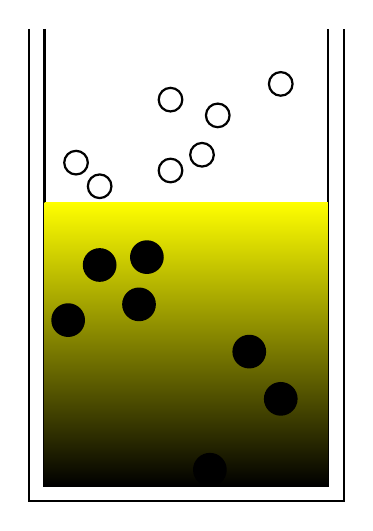
\begin{tikzpicture}[thick]
\draw (0,6) -- (0,0) -- (4,0) -- (4,6);
\draw (0.2,6) -- (0.2,0.2) -- (3.8,0.2) -- (3.8,6);
\shade[top color=yellow, bottom color=black] (0.2,0.2) rectangle (3.8, 3.8);
\draw[black, fill=black](0.5, 2.3) circle(0.2);  
\draw[black, fill=black](1.5, 3.1) circle(0.2);  
\draw[black, fill=black](3.2, 1.3) circle(0.2);  
\draw[black, fill=black](2.3, 0.4) circle(0.2);  
\draw[black, fill=black](1.4, 2.5) circle(0.2);  
\draw[black, fill=black](0.9, 3.0) circle(0.2);  
\draw[black, fill=black](2.8, 1.9) circle(0.2);  

\draw[black](0.6, 4.3) circle(0.15);  
\draw[black](1.8, 5.1) circle(0.15);  
\draw[black](3.2, 5.3) circle(0.15);  
\draw[black](2.2, 4.4) circle(0.15);  
\draw[black](1.8, 4.2) circle(0.15);  
\draw[black](0.9, 4.0) circle(0.15);  
\draw[black](2.4, 4.9) circle(0.15);      
%\node [rectangle, draw, rotate=45]{};
\end{tikzpicture}
\caption{The presence of a solute reduces the boiling point of the solvent.}
\label{boil}
\end{figure}

